\section{Syslog}

\subsection{Syslog Server Setup}

To have a centralized logging system, a syslog server is needed. This server will collect all the logs from the different devices and store them in a central location and make them available for analysis and monitoring.\\
After doing some research on the internet, I found that \textit{Graylog Open} is a popular solution for this task. It is open-source and has a lot of features that make it a great tool for this job.\\
The easiest way to set up a Graylog server is to use the provided Docker container. This will be achieved using the Portainer CE interface.\\
For this a new stack has to be created in Portainer CE. The stack will be named \textit{graylog} and will contain the sample docker-compose file provided by the Graylog documentation.\\ 
\url{https://github.com/Graylog2/docker-compose/tree/main/open-core}\\
Additionally, the environment variables have to be set accordingly.

After configuring the stack the "Deploy the stack" button has to be pressed and the Graylog server will be deployed.

To finnish the initial setup some certificates have to be generated and the nodes have to be connected. This is easily done in the Graylog initialization web interface.
\begin{figure}[H]
	\centering
	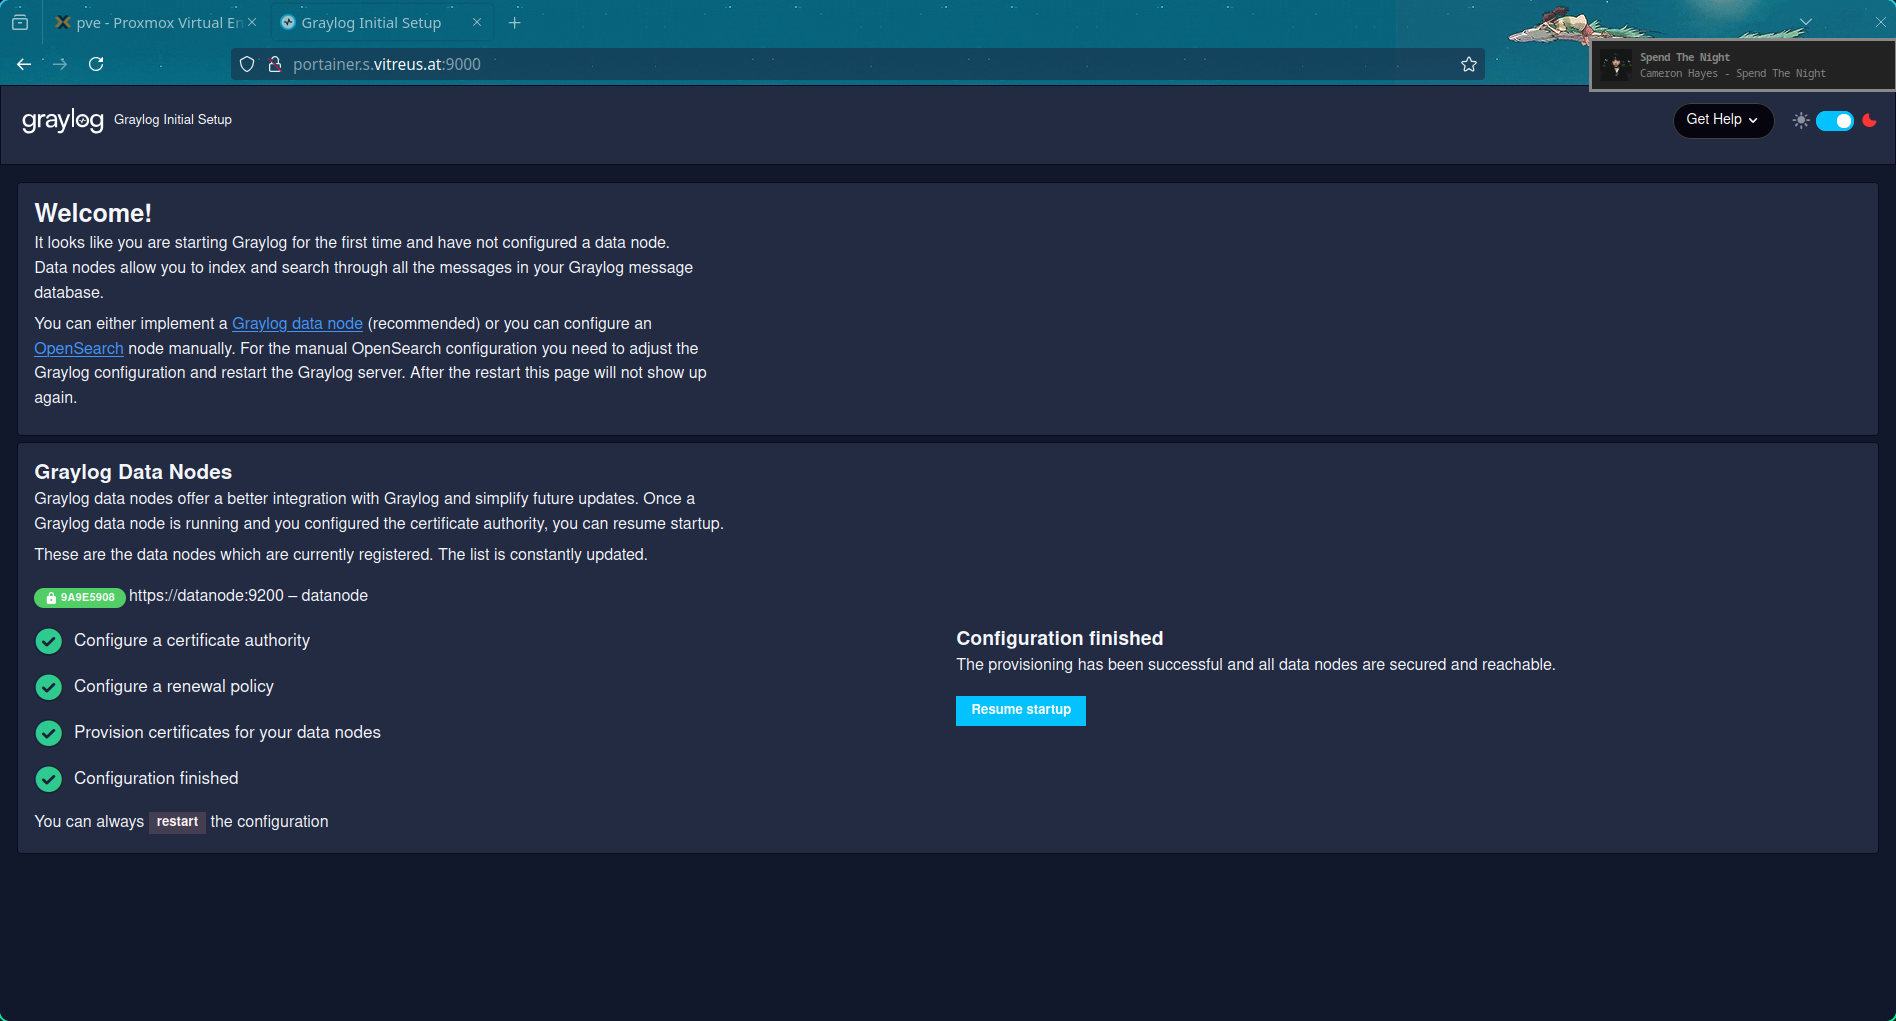
\includegraphics[width=0.8\linewidth]{Figures/graylog-initial-setup.png}
	\caption{Graylog initial setup}
\end{figure}
After the setup is done, the Graylog server is ready to receive logs from the different devices.


\begin{minted}{docker}
    ports:
    - "5044:5044/tcp"   # Beats
    - "5140:5140/udp"   # Syslog
    - "5140:5140/tcp"   # Syslog
    - "5555:5555/tcp"   # RAW TCP
    - "5555:5555/udp"   # RAW UDP
    - "9000:9000/tcp"   # Server API
    - "12201:12201/tcp" # GELF TCP
    - "12201:12201/udp" # GELF UDP
    #- "10000:10000/tcp" # Custom TCP port
    #- "10000:10000/udp" # Custom UDP port
    - "13301:13301/tcp" # Forwarder data
    - "13302:13302/tcp" # Forwarder config    
\end{minted}

Greylog supports multiple input methods, like GELF, Syslog, Beats, etc. For this setup, the Syslog input will be used. \\
To actually be able to receive logs, the input has to be started in the Graylog web interface. This can be done in the System $\rightarrow$ Inputs section.\\
Choose the input \textit{Syslog UDP}, name it, set the correct port, check the other config options and start the input.
\begin{figure}[H]
	\centering
	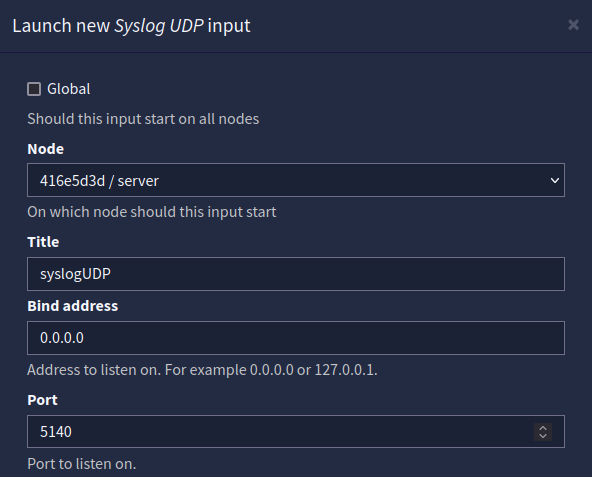
\includegraphics[width=0.8\linewidth]{Figures/syslog-udp-input.png}
	\caption{Creating a Syslog UDP input}
\end{figure}

After the input is started, the Graylog server is ready to receive logs from the different devices.

\subsection{Syslog Client Configuration}

Logs should be sent to the Graylog server from the different devices. This can be achieved by configuring the syslog daemon on the devices to send the logs to the Graylog server.

\subsubsection{Proxmox VE}

The first client that will be configured is the Proxmox server. This can be done by editing the \textit{/etc/rsyslog.conf} file. The following lines have to be added to the file:
\begin{minted}{text}
# Graylog
*.* @graylog.s.vitreus.at:5140
\end{minted}
This will send all logs to the Graylog server. After saving the file the rsyslog service has to be restarted using \mintinline{bash}|systemctl restart rsyslog.service|

After some time logs should start to appear in the Graylog web interface.
\begin{figure}[H]
	\centering
	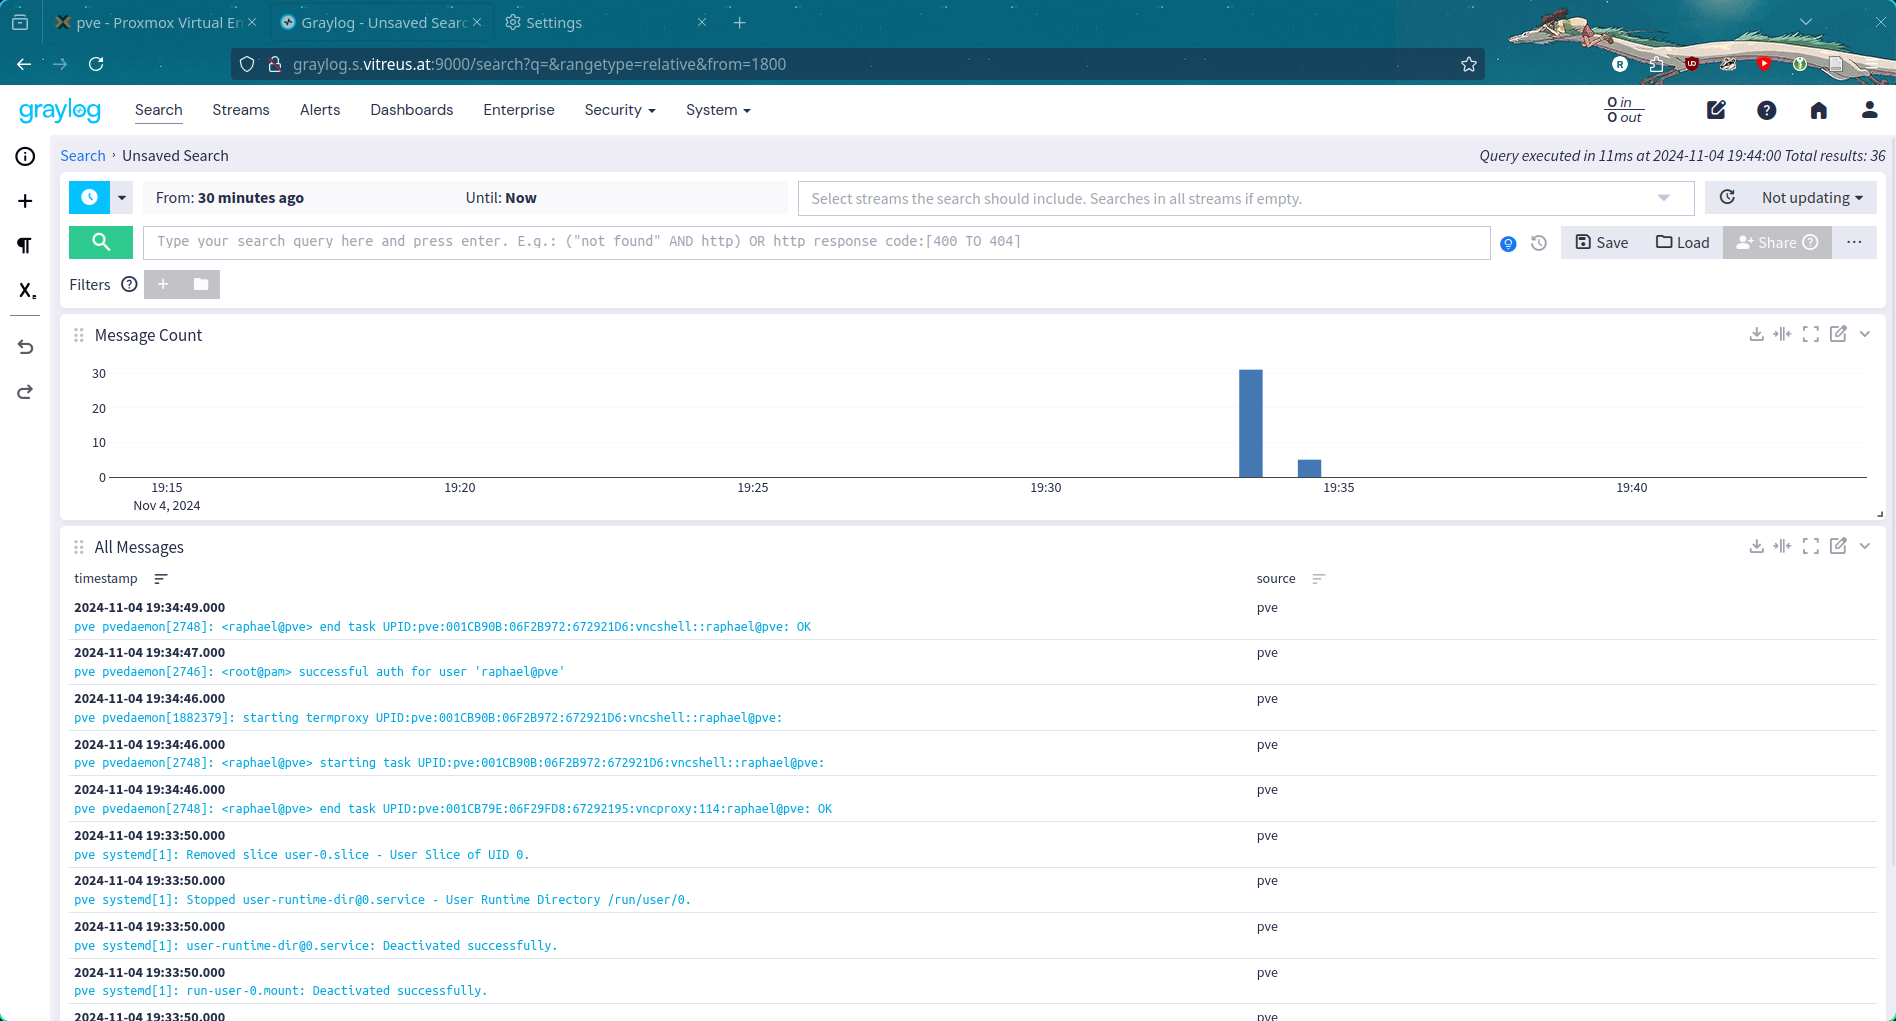
\includegraphics[width=1\linewidth]{Figures/graylog-search-example-proxmox.png}
	\caption{Proxmox logs in Graylog}
\end{figure}

\subsubsection{OPNsense Firewall}

The second client that will be configured is a virtualized OPNsense firewall. This can be done by creating a remote syslog target in the OPNsense web interface under System $\rightarrow$ Settings $\rightarrow$ Logging $\rightarrow$ Remote.


\begin{figure}[H]
	\centering
	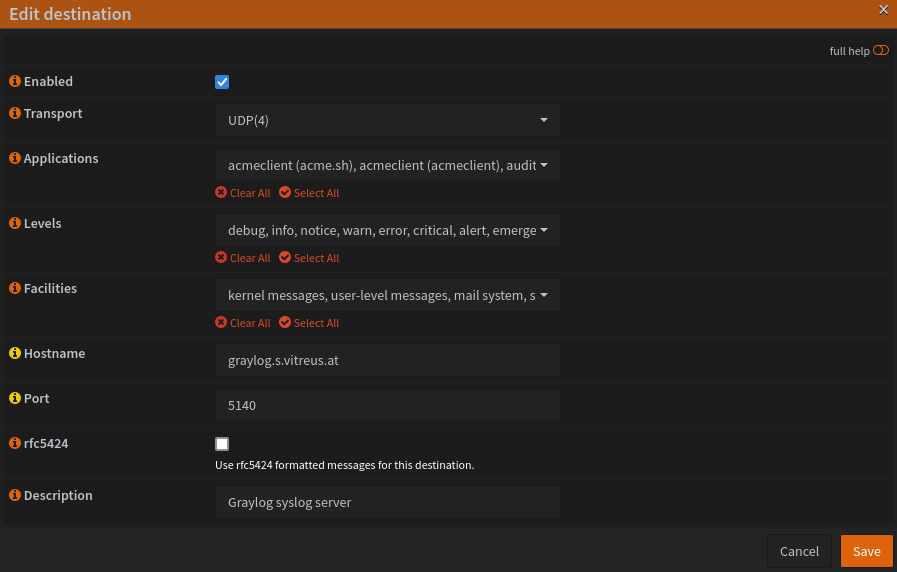
\includegraphics[width=0.8\linewidth]{Figures/opnsense-syslog-target.png}
	\caption{OPNsense remote syslog target}
\end{figure}
The web interface allows you to select specific applications, level or facilities to send to the remote syslog server. For this example, all logs will be sent to the Graylog server.

After hitting the save button and applying the changes, logs should start to appear in the Graylog web interface.

\begin{figure}[H]
	\centering
	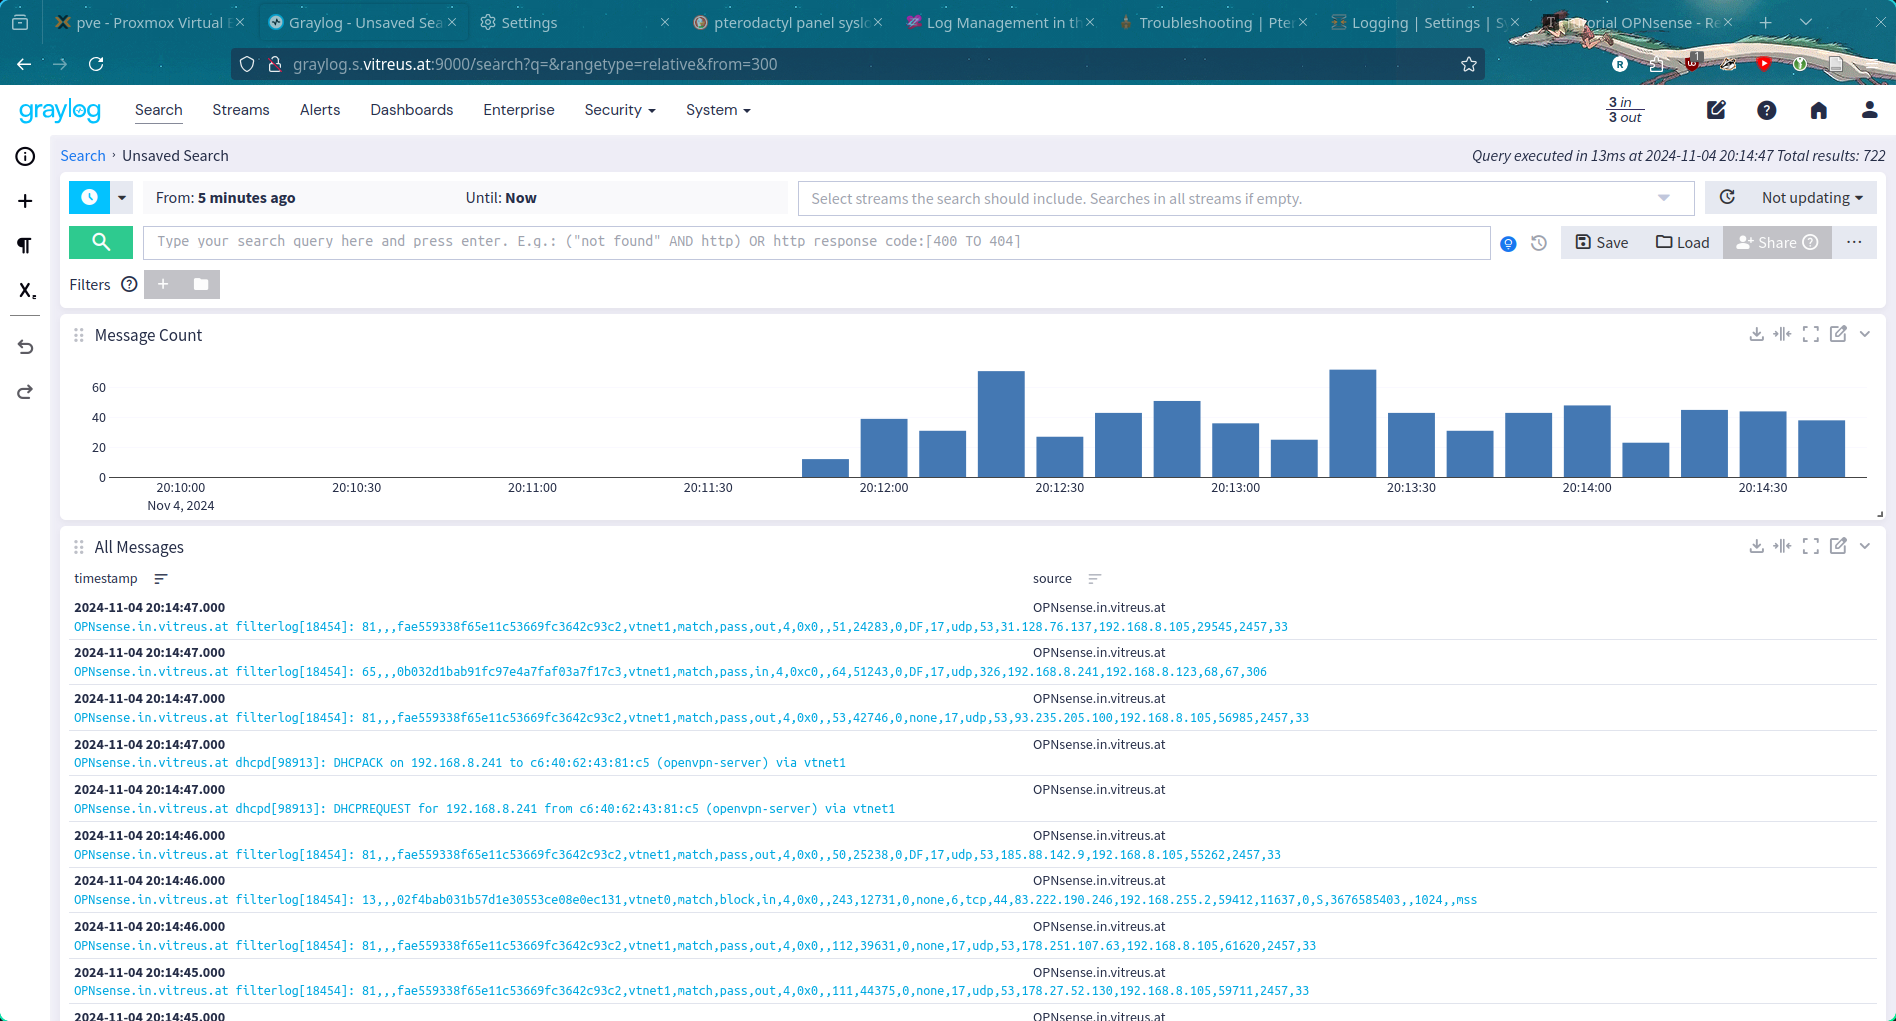
\includegraphics[width=1\linewidth]{Figures/graylog-search-example-opnsense.png}
	\caption{OPNsense logs in Graylog}
\end{figure}

\subsection{NTP}

To have a consistent time on all devices, it is a good idea to use NTP. 

\textbf{Proxmox VE} runs \textit{chrony} as an NTP client by default. The configuration can be found in the \textit{/etc/chrony/chrony.conf} file. It is configured to use a pool of global time-servers. The default configuration should be sufficient for most use cases.

\textbf{OPNsense} also runs an NTP service by default. The configuration can be found in the web interface under Services $\rightarrow$ Network time $\rightarrow$ General. It uses a pool of 4 opnsense time servers by default.
\begin{figure}[H]
	\centering
	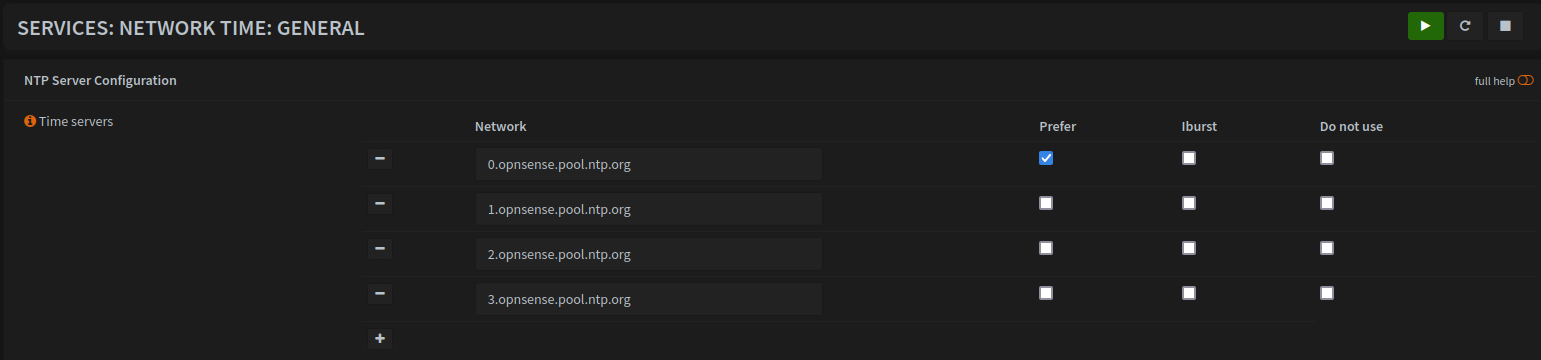
\includegraphics[width=1\linewidth]{Figures/opnsense-ntp.png}
	\caption{OPNsense Network Time}
\end{figure}

\subsection{Message Types}

Syslog messages are divided into 8 severity levels and 23 facility codes. The severity levels are:
\begin{itemize}
    \item Emergency (0)
    \item Alert (1)
    \item Critical (2)
    \item Error (3)
    \item Warning (4)
    \item Notice (5)
    \item Informational (6)
    \item Debug (7)
\end{itemize}
The facility codes are:
\begin{itemize}
    \item Kernel messages (0)
    \item User-level messages (1)
    \item Mail system (2)
    \item System daemons (3)
    \item Security/authorization messages (4)
    \item Messages generated internally by syslogd (5)
    \item Line printer subsystem (6)
    \item Network news subsystem (7)
    \item UUCP subsystem (8)
    \item Clock daemon (9)
    \item Security/authorization messages (10)
    \item FTP daemon (11)
    \item NTP subsystem (12)
    \item Log audit (13)
    \item Log alert (14)
    \item Clock daemon (15)
    \item Local use 0-7 (16-23)
\end{itemize}

The severity levels are used to indicate the importance of the message. The facility codes are used to indicate the source of the message.

\subsection{Syslog Sniffing}

To see how syslog messages are sent and received, a network sniffer (e.g. Wireshark, tshark) can be used. 

To capture syslog messages tshark was installed on Proxmox:\\
\mintinline{bash}|apt install tshark|

To capture traffic for 30 seconds on \textit{vmbr0} and save it to a file, the following command was used:\\
\mintinline{bash}|tshark -i vmbr0 -a duration:60 -w capture_output.pcap|

The resulting pcap file can be opened in Wireshark to analyze the captured traffic.

\begin{figure}[H]
	\centering
	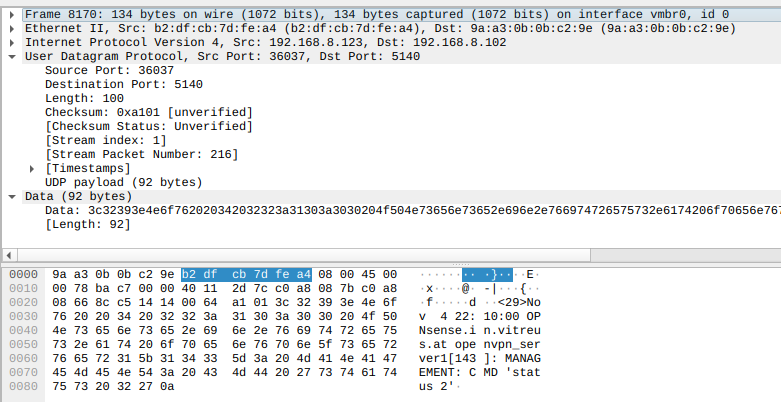
\includegraphics[width=1\linewidth]{Figures/wireshark-syslog.png}
	\caption{Wireshark syslog capture}
\end{figure}

\textbf{Syslog Message Example:}
\begin{minted}{text}
<29>Nov  4 22:10:00 OPNsense.in.vitreus.at openvpn_server1[143]: MANAGEMENT: CMD 'status 2'
\end{minted}

\bigskip
\noindent
\textbf{Syslog Message Components:}

\begin{enumerate}
    \item \textbf{Priority Value} \texttt{<29>} \\
    The priority value, \texttt{<29>}, encodes both the facility and severity levels based on Syslog standards.

    \item \textbf{Timestamp} \texttt{Nov 4 22:10:00} \\
    The date and time the message was generated. Here, it shows November 4 at 22:10:00.

    \item \textbf{Hostname} \texttt{OPNsense.in.vitreus.at} \\
    Identifies the source system that generated the log.

    \item \textbf{Application Name} \texttt{openvpn\_server1[143]} \\
    The program or process that generated the message, with \texttt{[143]} representing the process ID.

    \item \textbf{Message Content} \texttt{MANAGEMENT: CMD 'status 2'} \\
    Provides details about the event, in this case showing a command issued by the OpenVPN management interface.
\end{enumerate}
